\documentclass[11pt]{article}

% ============ arXiv-standard packages ============
\usepackage[margin=1in]{geometry}
\usepackage{times}
\usepackage[T1]{fontenc}
\usepackage[utf8]{inputenc}
\usepackage{graphicx}
\usepackage{booktabs}
\usepackage{multirow}
\usepackage{amsmath,amssymb}
\usepackage{hyperref}
\usepackage[capitalize]{cleveref}
\usepackage{authblk}
\usepackage{caption}
\usepackage{xcolor}
\usepackage{enumitem}

\hypersetup{
    colorlinks=true,
    linkcolor=blue,
    citecolor=blue,
    urlcolor=blue,
    pdftitle={Are Real-World SBOMs Ready for the EU Cyber Resilience Act?},
    pdfauthor={Hrishikesh Kanapuram}
}

\title{Are Real-World SBOMs Ready for the EU Cyber Resilience Act?\\
\large A Large-Scale Empirical Study of CRA Annex I Compliance Across 5,000 Software Bills of Materials}

\author[1]{Hrishikesh Kanapuram}
\affil[1]{Symbiosis Skills and Professional University\\\texttt{hrishik10@student.sspu.ac.in}}

\date{June 2026}

\begin{document}

\maketitle

\begin{abstract}
The EU Cyber Resilience Act (CRA) introduces security-disclosure requirements for Software Bills of Materials (SBOMs) that go substantially beyond the NTIA Minimum Elements used as the compliance benchmark in prior work. CRA Article 13's SBOM obligations take effect in September 2026, yet it remains unclear whether SBOMs produced by current open-source tooling -- the tooling most manufacturers will rely on to meet this obligation -- satisfy these additional requirements by default. We address this question empirically, using a random sample of 5,000 SBOMs from the Wild SBOMs dataset -- itself mined from 78,612 files across 1,782 code-hosting forges. We evaluate each file against a 19-check taxonomy spanning NTIA-equivalent presence checks, CRA-specific requirements, general SBOM-quality checks, and checks conditional on the presence of vulnerability data. NTIA-equivalent checks pass at an average rate of 77.0\%, while the four checks most directly grounded in CRA Annex I's vulnerability-handling, lifecycle, and support-period obligations pass at just 4.9\% -- a gap of 72.2 percentage points (Wilcoxon signed-rank test, $p<0.001$). This gap is stable across extensive sensitivity analysis: even when the three largest tool categories are excluded, or when the corpus is restricted to tools each contributing under 5\% of files, the gap remains within 65.6--72.2 percentage points. The vulnerability-disclosure gap -- the most operationally demanding of CRA's additional requirements -- is driven not by poor data quality but by near-total absence: only 0.32\% of SBOMs provide structured, machine-readable vulnerability data, though among the small number that do, most use recognisable identifier formats and validate against OSV.dev. We additionally find that mainstream tools (e.g., trivy) are capable of producing CRA-relevant structured output, suggesting the gap reflects adoption and configuration choices rather than a lack of tooling capability. Consistency across such tools, however, remains an open question. We provide a dated pre-enforcement baseline, drawn from SBOMs collected through approximately October 2024 and evaluated in June 2026, along with remediation priorities for the September 2026 deadline.
\end{abstract}

\textbf{Keywords:} Software Bill of Materials, SBOM, Cyber Resilience Act, CRA, NTIA Minimum Elements, CycloneDX, SPDX, empirical study, vulnerability disclosure, supply-chain security

\section{Introduction}
\label{sec:introduction}

Software Bills of Materials (SBOMs) have moved from a niche supply-chain artifact to a regulatory requirement. In the United States, Executive Order 14028 (2021) drove adoption of the National Telecommunications and Information Administration's (NTIA) Minimum Elements for a Software Bill of Materials, a seven-field baseline (component name, version, supplier, unique identifiers, dependency relationships, SBOM author, and timestamp) intended to make software composition machine-readable and auditable. In the European Union, the Cyber Resilience Act (CRA) goes considerably further: Annex I imposes security-relevant obligations -- including vulnerability handling, component end-of-life status, and security support periods -- that have no direct counterpart in NTIA's original seven fields. CRA Article 13's SBOM-related obligations take effect in September 2026, with full enforcement following in December 2027. The research community has already begun grappling with the scale of this transition: a 2024 Dagstuhl seminar convened CRA experts from policy, industry, and academia to identify open research challenges in standardisation, developer practice, and empirical measurement of compliance readiness \cite{dagstuhl2024}.

This raises an empirical question: to what extent does the output of current, widely-used open-source SBOM tooling satisfy CRA Annex I's additional requirements, as opposed to the NTIA baseline alone? Despite a growing body of empirical work measuring SBOM quality and completeness (see \cref{sec:related}), no existing study answers this question directly. Prior work either measures against NTIA's Minimum Elements, against generic format-quality scores (e.g., via sbomqs), against binary-level dependency accuracy \cite{jbomaudit}, or -- in the cases that engage with CRA text directly \cite{corti2025,ruohonen2025timmers,ruohonen2025gdpr} -- does so qualitatively or at the regulatory-mapping level, without an SBOM corpus to validate against.

We address this gap directly. Using a random sample of 5,000 SBOM files drawn from the Wild SBOMs dataset \cite{soeiro2025} -- itself mined from over 78,000 SBOMs across 1,782 code-hosting forges via the Software Heritage Archive -- we evaluate each file against a 19-check taxonomy spanning data presence, data quality, and contextual/operational requirements. Because the corpus is drawn from public code-hosting platforms, it predominantly captures open-source, developer-facing SBOMs rather than the confidential, manufacturer-internal SBOMs that CRA Article 13 directly governs; we treat our findings as a measurement of what current open-source tooling produces by default -- the tooling base that most manufacturers, including those building CRA-regulated products, are likely to build upon or adapt. We organise the 19 checks into four requirements groups: nine NTIA-equivalent checks, four CRA-specific checks, three general SBOM-quality checks (component integrity hashing, licence presence, and licence validity), and two checks conditional on the presence of structured vulnerability data. The full mapping and rationale for each group are given in \cref{sec:taxonomy}.

Our central finding is a substantial compliance gap. Across the corpus, the NTIA-equivalent checks pass at an average rate of 77.0\%, while the four CRA-specific checks pass at an average rate of just 4.9\% -- a gap of 72.2 percentage points, which a Wilcoxon signed-rank test on per-SBOM pass rates confirms is statistically significant ($p<0.001$, $n=4{,}999$). This gap is highly stable: across a range of sensitivity analyses excluding the largest tool categories individually and cumulatively, and when restricting the corpus to tools each contributing under 5\% of files, the gap remains between 65.6 and 72.2 percentage points. In other words, SBOMs being produced by today's open-source tooling are, on average, reasonably well-aligned with a five-year-old US baseline, but substantially unprepared for the additional security-disclosure obligations the EU's CRA will require -- with particular gaps in vulnerability declaration, component end-of-life status, and deployment-context disclosure.

A second finding concerns why the gap exists, rather than merely its size. CRA Annex I's vulnerability-handling requirements are arguably its most operationally demanding: they require manufacturers to identify and address known vulnerabilities in included components, and we interpret structured, machine-actionable data as the practical mechanism for doing so at scale. We find that only 16 of 5,000 SBOMs (0.32\%) provide this kind of structured, machine-readable vulnerability data within the SBOM itself. Among those 16 SBOMs, most use a recognisable vulnerability-identifier format and validate against the OSV.dev database, though this sub-finding rests on a small sample (95\% CI: 50.5--89.8\%) and should be treated as provisional. This suggests the CRA vulnerability-disclosure gap is, at present, predominantly a problem of absence -- tools are not populating these fields at all -- rather than a problem of quality among the small fraction of SBOMs that attempt it. Authoritative CRA implementation guidance, including Germany's BSI TR-03183-2, indicates that vulnerability disclosure may instead be intended to occur via separate VEX/CSAF documents rather than embedded within the SBOM itself \cite{bsi2025}; we discuss this architectural question in \cref{sec:cra-background} and revisit it when interpreting our findings in \cref{sec:discussion}.

We make the following contributions:

\begin{enumerate}
\item To the best of our knowledge, the first empirical study to evaluate a corpus of real-world SBOMs against a taxonomy explicitly operationalised from CRA Annex I's requirements, as distinct from the NTIA Minimum Elements or generic format-quality scores that prior work has used as its benchmark.
\item A 19-check taxonomy mapping individual, automatable checks to NTIA fields, CRA-specific requirements, general SBOM-quality properties, and a ``conditional on presence'' category for vulnerability-quality measures that only apply when vulnerability data exists at all.
\item A quantified pre-enforcement baseline (77.0\% / 4.9\% / 72.2pp gap) drawn from SBOMs collected through approximately October 2024 and evaluated in June 2026, against which post-CRA-enforcement SBOM practice can be compared in future work.
\item A presence-versus-quality decomposition of the vulnerability-disclosure gap, including a tool-capability analysis identifying generators that already produce CRA-relevant structured vulnerability output -- a finding we interpret cautiously given recent evidence of substantial inconsistency across vulnerability-scanning tools \cite{churakova2025}.
\end{enumerate}

The remainder of this paper is organised as follows. \Cref{sec:background} provides background on CRA Annex I and NTIA's Minimum Elements, and on the SPDX and CycloneDX SBOM formats. \Cref{sec:related} situates our work relative to existing empirical SBOM-quality literature. \Cref{sec:methodology} describes our dataset, sampling methodology, and 19-check taxonomy. \Cref{sec:results} presents our results. \Cref{sec:discussion} discusses remediation implications. \Cref{sec:threats} addresses threats to validity, and \Cref{sec:conclusion} concludes.

\section{Background}
\label{sec:background}

\subsection{SBOM Formats: SPDX and CycloneDX}

A Software Bill of Materials is a structured, machine-readable inventory of the components -- libraries, packages, modules -- that make up a piece of software, along with metadata describing those components and their relationships. Two formats dominate current practice.

SPDX (Software Package Data Exchange) originated in the open-source license-compliance community and became an ISO/IEC standard (ISO/IEC 5962:2021). It is document-centric: an SPDX file describes a set of packages, each with fields such as name, version, supplier, originator, licence information, and external references, plus relationships between packages.

CycloneDX originated within the OWASP community with an explicit security-tooling focus. It is distributed in JSON or XML and organises a components array (each with name, version, supplier/publisher, package URLs, and licences) alongside top-level metadata (authorship, timestamp, tool information) and, notably, an optional vulnerabilities array intended to carry structured, per-component vulnerability disclosures -- a feature with no direct SPDX equivalent prior to SPDX 2.3's more limited security-related fields.

Both formats remain in active use across the open-source SBOM-tooling ecosystem, and their differing field support has direct consequences for the checks in our taxonomy: several CRA-relevant checks depend on CycloneDX-specific fields with no SPDX counterpart in the format versions evaluated in this study (\cref{sec:taxonomy}). The corpus's format distribution is reported in \cref{sec:sampling}.

\subsection{NTIA Minimum Elements}

In response to US Executive Order 14028 (May 2021), NTIA published ``The Minimum Elements For a Software Bill of Materials'' \cite{ntia2021}, defining a baseline of seven required data fields that any SBOM should contain regardless of format. Three identify the component itself: Supplier Name, Component Name, and Component Version. A fourth, Other Unique Identifiers (e.g., PURL, CPE), supplements this with machine-resolvable identity. A fifth, Dependency Relationship, captures structure; the remaining two, Author of SBOM Data and Timestamp, establish provenance.

NTIA additionally specifies ``automation support'' guidance -- that SBOMs be produced in a machine-readable format (SPDX, CycloneDX, or SWID) with the format version identified -- though this is framed as a practice recommendation rather than an additional data field. NTIA's 2021 Minimum Elements are deliberately format-agnostic and presence-oriented: they ask whether a field exists, not whether its content meets any particular quality bar beyond that. They also predate, and do not address, security-disclosure content such as known vulnerabilities, component lifecycle status, or support periods.

CISA released draft updated minimum elements in August 2025 \cite{cisa2025}, proposing several additional fields -- including component cryptographic hashes and licence information -- that were not part of the original 2021 baseline; public comment on this draft closed in October 2025, and at the time of writing it has not been confirmed as finalised. Two of our taxonomy's checks (component integrity hashing and licence presence; \cref{sec:taxonomy}) anticipate elements proposed in this draft. We retain the 2021 baseline as our primary point of comparison throughout this paper, since it remains the only finalised NTIA reference, but report these two checks separately from our core NTIA-equivalent group (rather than folding them into either the 2021 baseline or our CRA-specific group) given their uncertain regulatory status as of this writing.

\subsection{CRA Annex I}
\label{sec:cra-background}

The EU Cyber Resilience Act (Regulation (EU) 2024/2847) \cite{cra2024} establishes cybersecurity requirements for products with digital elements placed on the EU market. Annex I, Part I sets out essential security requirements that manufacturers must address throughout a product's lifecycle, and Article 13 establishes corresponding obligations including the maintenance of an SBOM covering, at minimum, the top-level dependencies of the product. Ruohonen et al. \cite{ruohonen2025gdpr} provide a detailed mapping of CRA's essential requirements, identifying the SBOM obligation and vulnerability-coordination obligations as two distinct provisions among CRA's seven new essential requirements -- a distinction we return to below.

Critically, CRA's security requirements extend well beyond NTIA's component-inventory framing into the operational security posture of the components listed. Three obligations recur across this substantive layer, and each is the focus of one or more checks in our taxonomy: identifying and addressing known vulnerabilities in included components, ensuring components are not running unsupported or end-of-life versions, and documenting the security-support timeline for components and the product as a whole. None of these obligations have a direct equivalent among NTIA's seven Minimum Elements. An SBOM that fully satisfies NTIA -- every component named, versioned, identified, related, authored, and timestamped -- could still be entirely silent on whether any of those components have known vulnerabilities, are end-of-life, or have a defined support window. It is precisely this additional layer of requirements that our 19-check taxonomy (\cref{sec:methodology}) is designed to separate out and measure.

\textbf{A question we treat with particular care throughout this paper concerns \emph{where} vulnerability information is intended to reside -- within the SBOM itself, or in an accompanying document.} CRA Annex I's text does not prescribe that vulnerability data be embedded within the SBOM document itself, and the regulation's broader vulnerability-coordination obligations are arguably satisfied through a separate disclosure mechanism. Ruohonen and Timmers \cite{ruohonen2025timmers} analyse CRA's vulnerability-coordination requirements in detail and distinguish them from the SBOM obligation proper. More concretely, Germany's Federal Office for Information Security (BSI), in its technical guideline TR-03183-2 -- currently the most detailed published implementation guidance for CRA's SBOM obligations -- treats the SBOM and the vulnerability disclosure as two separate artefacts: known vulnerabilities are reported through Vulnerability Exploitability eXchange (VEX) or Common Security Advisory Framework (CSAF) documents, while the SBOM itself need not carry this data \cite{bsi2025}. Under this reading, an SBOM could be fully CRA-compliant with respect to vulnerability handling while containing no vulnerability data at all, provided the manufacturer maintains and references the required VEX/CSAF documentation separately.

We do not adopt this narrower reading as our primary framing. CRA's regulatory text itself remains the binding instrument, and BSI TR-03183-2 represents one national authority's implementation guidance rather than a definitive pan-EU interpretation; other member states' technical guidance may differ, and may evolve as enforcement approaches. Moreover, regardless of whether vulnerability data is required inside the SBOM specifically or in an accompanying VEX/CSAF document, a structured and machine-readable representation of known vulnerabilities is necessary for CRA compliance at scale under either reading -- and measuring whether SBOMs themselves carry this information remains informative, since SBOM-embedded data is one of the two mechanisms by which it could be satisfied, and the one most directly comparable to NTIA's SBOM-centric framing. We nonetheless flag this architectural question explicitly here, revisit it when defining our vulnerability-related checks in \cref{sec:taxonomy}, and discuss its implications for interpreting our results in \cref{sec:discussion}.

\subsection{Why the Gap Matters Now}

CRA Article 13's SBOM-related obligations take effect in September 2026 -- at the time of writing (June 2026), approximately three months away -- with the regulation's full enforcement regime following in December 2027. The tooling ecosystem that generates SBOMs today (cdxgen, syft, language-specific generators such as cyclonedx-php-composer and cyclonedx-gomod, and others) was, for the most part, built and configured against the NTIA baseline and general SPDX/CycloneDX schema conformance -- not against CRA Annex I's specific additional content requirements. Whether that tooling's default output already happens to satisfy CRA's additional requirements, or whether a substantial configuration and tooling effort is needed before September 2026, is an empirical question this paper answers.

\section{Related Work}
\label{sec:related}

A growing body of empirical and regulatory-analysis work bears on the question we ask in this paper. \Cref{tab:related-work} summarises 25 studies relevant to ours, spanning empirical SBOM measurement, tool-adherence analysis, practitioner surveys, vulnerability-tooling consistency, and CRA regulatory interpretation. Across the empirical literature specifically, a consistent pattern emerges: every study that measures SBOM quality against a concrete benchmark does so using NTIA's Minimum Elements, generic format-level quality scores, or binary-level dependency accuracy -- not CRA Annex I as the measurement benchmark.

\paragraph{NTIA-completeness and accuracy studies.} Muneza et al.\ \cite{muneza2025} analysed 2,225 Docker images across four corpora, measuring how SBOM generation tool and output format affect compliance with NTIA's Minimum Elements, finding substantial tool-to-tool variation. Nocera et al.\ \cite{nocera2025jss} mined 186 open-source GitHub repositories, measuring SBOM adoption trends, update frequency, and information completeness against NTIA's minimum and recommended fields -- a longitudinal dimension absent from our single-snapshot study. Across four languages (Python, C, Rust, TypeScript), Halbritter and Merli \cite{halbritter2024} found that no SBOM tool fully satisfies all NTIA requirements in any language, and called for more precise government-issued accuracy specifications; this finding anticipates our own supplier-identification result (\cref{sec:a3-discussion}). Most directly relevant to our presence-based design choice, Xiao et al.\ \cite{jbomaudit} introduce JBomAudit, which moves beyond presence-checking to measure binary-level \emph{correctness} of declared dependencies in 25,882 Java SBOMs against ground-truth JAR contents, finding 7,907 SBOMs omit direct dependencies entirely. Our taxonomy deliberately measures field \emph{presence} rather than binary-level correctness, since CRA Annex I's text concerns whether information is disclosed at all rather than its downstream accuracy; JBomAudit's findings nonetheless suggest that even where our checks register a PASS, the underlying content may not always be fully accurate -- a limitation we discuss in \cref{sec:threats}.

\paragraph{Large-scale tool-adherence and consistency studies.} The largest study in this space is Wang et al.'s \cite{wang2026} analysis of 55,444 SBOMs across 3,287 repositories, which measures both schema-level adherence to the SPDX/CycloneDX specifications and, separately, a degree of NTIA policy-field compliance; we engage with this distinction below. Wu et al.\ \cite{wu2025} constructed a 152-project Java benchmark for evaluating SBOM tools, using NTIA requirements alongside a CRA-informed framing without empirically measuring CRA-specific content. A differential analysis by Yu et al.\ \cite{yu2024} of four major SBOM generators (including trivy and syft, both prominent in our own corpus) across 7,876 repositories spanning nine languages found that all four produce inconsistent and incomplete output relative to one another -- a finding we revisit in \cref{sec:tool-format} when interpreting tool-level differences in our results. Rabbi et al.\ \cite{rabbi2025} extended this line of work to the Rust ecosystem, comparing claimed versus actual tool capability across seven generators and finding substantial gaps, relevant to interpreting cyclonedx-gomod's low scores in our corpus. The most comprehensive recent ecosystem-level comparison is Bangash et al.'s \cite{bangash2026} analysis of 170 SBOM tools and 36,990 issue reports across the CycloneDX and SPDX communities, which finds that CycloneDX tooling shows higher developer engagement while the SPDX ecosystem offers broader tool availability -- context relevant to the format-level differences we report in \cref{sec:tool-format}.

\paragraph{Vulnerability and VEX tooling consistency.} Closely related to our vulnerability-disclosure findings (\cref{sec:a8-decomp,sec:conditional}), Churakova et al.\ \cite{churakova2025} systematically evaluate seven VEX-generation tools -- including trivy, the tool we identify in \cref{sec:existence-proof} as capable of producing CRA-relevant structured vulnerability output -- and find low cross-tool consistency (maximum pairwise Jaccard similarity of 69.4\%, driven primarily by differences in the underlying vulnerability databases each tool queries). This finding directly qualifies how we interpret tool capability in \cref{sec:existence-proof,sec:discussion}: a tool's demonstrated ability to produce CRA-relevant output does not establish that such output is consistent or complete relative to other capable tools.

\paragraph{Dataset construction and practitioner-perspective studies.} The source of our corpus, Soeiro et al.\ \cite{soeiro2025}, contributed the Wild SBOMs dataset of 78,612 real-world SBOMs, annotated with generic quality scores via sbomqs, and explicitly proposed CRA-style compliance assessment as a use case for future work without performing it themselves; our paper directly takes up this proposal. O'Donoghue et al.\ \cite{odonoghue2024} examined how SBOM generation choices affect downstream vulnerability detection across 2,313 Docker images. Novikov et al.\ \cite{novikov2025} studied 620 policy-driven SBOMs from GitHub using generic sbomqs scoring. Two studies survey SBOM practitioners directly: Xia et al.\ \cite{xia2023} combined 17 interviews with a 65-respondent survey on SBOM practice broadly, while Stalnaker et al.\ \cite{stalnaker2024} substantially extended this with 138 respondents across five stakeholder groups (including AI/ML, cyber-physical systems, and legal practitioners) and follow-up interviews, identifying 12 challenges spanning content deficiencies, tooling immaturity, and verification difficulties -- several of which (notably inaccurate/incomplete SBOMs and insufficient tooling) directly anticipate the gap we quantify empirically in \cref{sec:results}. Bi et al.\ \cite{bi2024} mined 4,786 GitHub discussions across 510 SBOM-related projects to characterise SBOM lifecycle challenges from a developer-discussion perspective, complementing Stalnaker et al.'s survey-based findings with naturally-occurring discourse data. A survey of Italian industry practitioners by Nocera et al.\ \cite{nocera2024icsme} found that SBOM adoption remains low despite awareness of supply-chain risk, attributing this partly to limited familiarity with emerging regulation including CRA -- a finding consistent with the adoption-gap interpretation we offer in \cref{sec:discussion}. Most recently, Zhang et al.\ \cite{zhang2026} provide a comprehensive cross-domain survey spanning SBOM, hardware, AI, and cryptographic bills of materials, situating SBOM-specific work such as ours within a broader BOM ecosystem.

\paragraph{CRA regulatory analysis.} Five works engage with CRA's text directly rather than empirically. Corti et al.\ \cite{corti2025} map CRA and NIS2 requirements text to open-source tooling capabilities qualitatively, without evaluating an SBOM corpus -- the regulatory scaffolding exists in this work, but not the empirical measurement we provide. Ruohonen and Timmers \cite{ruohonen2025timmers} and Ruohonen et al.\ \cite{ruohonen2025gdpr} analyse CRA's vulnerability-coordination and broader essential-requirements text in detail, respectively; we draw on both in \cref{sec:cra-background} to motivate our treatment of vulnerability disclosure as an architecturally contested question rather than a settled one. Complementing these academic analyses, BSI's TR-03183-2 \cite{bsi2025} provides the most detailed published national implementation guidance for CRA's SBOM obligations to date; we engage with it directly in \cref{sec:cra-background,sec:taxonomy}. A 2024 Dagstuhl seminar \cite{dagstuhl2024} further reflects the broader research community's recognition that CRA compliance measurement -- including the empirical question this paper addresses -- remains an open area requiring sustained attention. None of these five works evaluates an SBOM corpus against CRA Annex I requirements.

\paragraph{The gap.} Of the empirical studies surveyed, several cite CRA as motivating context, and one (Wu et al.\ \cite{wu2025}) adopts CRA-informed framing in its design, but none use CRA Annex I as the measurement benchmark against which SBOM content is directly evaluated. The five works that do engage with CRA text directly do so qualitatively or at the level of regulatory mapping, without an SBOM corpus. No existing study -- to the best of our knowledge -- answers the question: what fraction of SBOMs, as generated by current open-source tooling, would satisfy the content requirements introduced by CRA Annex I beyond the NTIA baseline?

Our work fills this gap directly. It is worth being precise about the distinction from Wang et al.\ \cite{wang2026}, the closest prior work in scale. Wang et al.\ measure two related but distinct things: the degree to which generated SBOMs conform to the SPDX/CycloneDX specifications themselves (a schema-adherence question), and, separately, a degree of compliance with NTIA policy-relevant fields. Neither of these measures CRA Annex I's additional content requirements -- vulnerability handling, component lifecycle status, and security-support documentation -- which have no NTIA counterpart and are the focus of our CRA-specific check group (\cref{sec:taxonomy}). Our contribution is therefore complementary to, rather than a re-derivation of, Wang et al.'s schema- and policy-adherence findings: we measure substantive CRA-specific disclosure content, regardless of underlying schema conformance.

\begin{table}[t]
\centering
\caption{Prior empirical SBOM-quality studies and CRA-relevant regulatory analyses. No prior study uses CRA Annex I as the measurement benchmark against an SBOM corpus.}
\label{tab:related-work}
\footnotesize
\begin{tabular}{p{0.04\textwidth}p{0.30\textwidth}p{0.32\textwidth}p{0.24\textwidth}}
\toprule
\# & Reference & Benchmark used & CRA role \\
\midrule
P1  & Xia et al., ICSE 2023 \cite{xia2023} & NTIA (citation only) & --- \\
P2  & Wang et al., TOSEM 2026 \cite{wang2026} & SPDX/CycloneDX spec adherence + NTIA policy compliance & Cited as context \\
P3  & Novikov et al., PROFES 2025 \cite{novikov2025} & Generic (sbomqs) & Cited as context \\
P4  & Muneza et al., SANER-C 2025 \cite{muneza2025} & NTIA Minimum Elements & --- \\
P5  & Wu et al., TOSEM 2025 \cite{wu2025} & NTIA + CRA-informed framing & Requirements framing \\
P6  & O'Donoghue et al., SCORED@CCS 2024 \cite{odonoghue2024} & None (vuln.\ detection impact) & --- \\
P7  & Corti et al., REW@ESPRE 2025 \cite{corti2025} & CRA + NIS2 (verbatim, qualitative) & Direct, no corpus \\
P8  & Soeiro et al., MSR 2025 \cite{soeiro2025} & Generic (sbomqs) & Cited as context; source of our corpus \\
P9  & Nocera et al., JSS 2025 \cite{nocera2025jss} & NTIA min + recommended & Cited as context \\
P10 & Stalnaker et al., ICSE 2024 \cite{stalnaker2024} & Survey (5 stakeholder groups) & Implicit -- regulatory pressure discussed \\
P11 & Xiao et al.\ (JBomAudit), NDSS 2025 \cite{jbomaudit} & NTIA accuracy + completeness (binary-level) & --- \\
P12 & Yu et al., DSN 2024 \cite{yu2024} & Differential tool-output analysis & --- \\
P13 & Churakova et al., arXiv 2025 \cite{churakova2025} & Jaccard/Tversky tool consistency & --- \\
P14 & Rabbi et al., SAC 2025 \cite{rabbi2025} & Precision/recall vs.\ ground truth & --- \\
P15 & Bi et al., TOSEM 2024 \cite{bi2024} & Mining GitHub discussions & --- \\
P16 & Ruohonen \& Timmers, ACIG 2025 \cite{ruohonen2025timmers} & CRA vulnerability-coordination analysis & Direct -- full analysis \\
P17 & Ruohonen et al., REW@RE 2025 \cite{ruohonen2025gdpr} & CRA + GDPR requirements mapping & Direct -- full CRA requirements enumeration \\
P18 & O'Donoghue et al., SLR 2025 \cite{odonoghue2025slr} & SLR of 40 SBOM studies & Cited as context \\
P19 & Bangash et al., arXiv 2025/26 \cite{bangash2026} & Ecosystem comparison (170 tools) & --- \\
P20 & Halbritter \& Merli, ARES 2024 \cite{halbritter2024} & NTIA accuracy across 4 languages & EU mentioned as motivation \\
P21 & Dagstuhl Seminar 24112 \cite{dagstuhl2024} & Expert seminar; no corpus & Direct -- full CRA framing \\
P22 & BSI TR-03183-2 v2.1.0 \cite{bsi2025} & Normative CRA SBOM field requirements & Direct implementation \\
P23 & SEI Plugfest Team, CMU/SEI SR-002 2025 \cite{seiplugfest2025} & Multi-tool comparison (170+ SBOMs) & Cited as context \\
P24 & Zhang et al., arXiv 2026 \cite{zhang2026} & Cross-domain BOM survey & Cited as context \\
P25 & CISA, draft 2025 \cite{cisa2025} & Updated NTIA minimum elements (draft) & Direct -- updates NTIA baseline \\
\bottomrule
\end{tabular}
\end{table}


\section{Methodology}
\label{sec:methodology}

We now describe the dataset, sampling procedure, and 19-check taxonomy used to operationalise this comparison.

\subsection{Dataset and Sampling}
\label{sec:sampling}

Our corpus is drawn from the Wild SBOMs dataset \cite{soeiro2025}, which mined 78,612 unique SBOM files from 94,618,356 repositories across 1,782 code-hosting forges via the Software Heritage Archive, with the underlying mining conducted through approximately October 2024. This provides a broad, multi-forge view of SBOM practice in the wild, in contrast to GitHub-only studies. As discussed in \cref{sec:introduction}, this corpus captures predominantly open-source, developer-facing SBOMs rather than the confidential, manufacturer-internal SBOMs that fall under CRA Article 13's direct scope; we treat it as a measurement of widely-used open-source tooling output rather than a sample of the CRA-regulated population itself.

From this archive, we drew a sample of 5,000 SBOM files meeting basic structural-validity criteria: a recognised format (CycloneDX-JSON, CycloneDX-XML, or SPDX-JSON), file size greater than 1\,KB, at least 5 declared components, and successful parsing. Sampling proceeded by shuffling the full file list and traversing it in the resulting order, stopping once 15,000 qualifying files had been identified (encountering 7,800 files rejected for the criteria above along the way, out of approximately 22,800 files examined in total); the first 5,000 files in this pre-shuffled, filtered sequence were retained as our analysis corpus. The shuffle was performed using Python's \texttt{random.shuffle()} without a fixed random seed; while the resulting 5,000-file sample is a valid random subset of the qualifying archive -- and we have no reason to expect it is unrepresentative -- it is not exactly reproducible, and an independent re-run of our sampling procedure would select a different, equally valid 5,000-file sample. We discuss this limitation further in \cref{sec:threats}.

One exception applies to CycloneDX-XML files: due to parser limitations at filtering time, the $\geq$5-component threshold was not enforced for this format; such files were instead accepted automatically with a placeholder component count (fixed at 99) and were not subject to tool-name extraction (discussed further in \cref{sec:threats}, Threat 8).

The resulting corpus consists of 4,412 CycloneDX-JSON files (88.2\%), 315 CycloneDX-XML files (6.3\%), and 273 SPDX-JSON files (5.5\%). Tool attribution was extracted from each SBOM's declared metadata: for CycloneDX, from the \texttt{metadata.tools} field; for SPDX, from \texttt{creationInfo.creators}. As reported, the corpus spans 54 distinct tool labels, the eight most frequent being cdxgen (1,348), ``Node.js module'' (917), cyclonedx-php-composer (623), cyclonedx-gomod (502), syft (445), unknown (346), Gemnasium (239), and Github Extractor (209), with the remaining 371 files spread across 46 additional labels.

\paragraph{Tool-attribution artifact.} A post-hoc audit of the ``Node.js module'' label revealed it to be a tool-attribution artifact rather than a genuine generator name. SBOMs using the CycloneDX 1.3/1.4 specification represent \texttt{metadata.tools} as a flat array of tool objects rather than the nested \texttt{tools.components} structure introduced in CycloneDX 1.5; for SBOMs produced by a tool that itself depends on the CycloneDX client library, the library's own self-declaration (``Node.js module'', contributed by the \texttt{@cyclonedx/cyclonedx-library} package) commonly appears as the first array entry, preceding the entry for the actual generating tool. Our tool-extraction logic selected the first array entry unconditionally, and therefore mislabelled these files. A diagnostic re-analysis of files carrying this label found the true generators were predominantly cdxgen (762 of 1,114 re-examined files, $\approx$68\%) and cyclonedx-php-composer (219 files, $\approx$20\%), with smaller contributions from Github Extractor under inconsistent capitalisation (131 files) and a small number of build-template artifacts (2 files). This means the true corpus share of cdxgen and cyclonedx-php-composer is materially higher than the figures reported above and used throughout \cref{sec:results}; we retain the original (mislabelled) attribution in all results tables for consistency, and report this as a limitation in \cref{sec:threats} rather than recomputing tool-level findings, since the affected analyses (\cref{sec:sensitivity}'s tool-concentration sensitivity analysis and \cref{sec:tool-format}'s per-tool breakdown) are not central to our headline NTIA-equivalent/CRA-specific gap, which is computed per-check across the full corpus independent of tool label.

\subsection{The 19-Check Taxonomy}
\label{sec:taxonomy-tiers}

We evaluate each SBOM against 19 automated checks, organised into three implementation tiers reflecting how each check is computed:

\begin{itemize}
\item \textbf{Tier A (13 checks, A1--A13):} core data-field presence and format-level requirements, evaluated directly from each SBOM's parsed structure without external queries.
\item \textbf{Tier B (4 checks, B1--B4):} data-quality and accuracy checks requiring cross-reference against external sources: vulnerability-identifier validation against OSV.dev (B1), component end-of-life status against the endoflife.date API (B2), PURL resolution against package-ecosystem registries (B3), and SPDX licence-identifier validity against the live SPDX licence list (B4).
\item \textbf{Tier C (2 checks, C1--C2):} structurally-inferred checks for which no standardised SBOM field exists, evaluated as multi-signal heuristics: deployment-environment inferability (C1) and security-support-period declaration (C2). Unlike Tier A/B checks, C1 and C2 return a binary PASS/FAIL based on the presence of \emph{any} qualifying signal among several candidate fields, rather than a per-component ratio; we treat this design choice as appropriate given that both checks assess a file-level property (does any such signal exist anywhere in the document) rather than a per-component one.
\end{itemize}

Each Tier A/B check returns PASS, PARTIAL, FAIL, or SKIP (where the underlying field or condition is not applicable to a given SBOM); Tier C checks return PASS or FAIL only. Pass rates are computed as the proportion of PASS results among non-SKIP evaluations. Separately from this implementation-tier structure, \cref{sec:taxonomy} below partitions the same 19 checks into four \emph{requirements groups} -- NTIA-equivalent, CRA-specific, general SBOM-quality, and conditional-on-presence -- according to which regulatory or quality framework each check measures. We draw this distinction explicitly because the two groupings do not align: for example, B4 (a Tier B data-quality check) belongs to the general-quality requirements group rather than the CRA-specific group, despite Tier B's name suggesting otherwise.

\subsection{Mapping Checks to NTIA, CRA, and General-Quality Requirements}
\label{sec:taxonomy}

To quantify the gap between established practice and CRA Annex I obligations, we partition the 19 checks into four requirements groups based on their correspondence to NTIA's 2021 Minimum Elements, to CRA-specific requirements not covered by NTIA, and to general SBOM-quality properties that, while valuable, are not uniquely attributable to either framework. This four-group partition reflects a correction identified during a later internal audit of the taxonomy's implementation: an earlier draft had placed three checks (A10, A11, B4) in the CRA-specific group based on Tier assignment alone, without verifying that their implementation logic measured CRA-specific content. We report only the corrected grouping throughout this paper.

\paragraph{NTIA-equivalent group (9 checks):} A1 (Component name), A2 (Component version), A3 (Supplier/originator), A4 (PURL/CPE identifier), A5 (Dependencies listed), A6 (SBOM author), A7 (Timestamp), A12 (Recognised SBOM format), and A13 (Format version declared).

Five of these (A1, A2, A3, A5, A6) map exactly to five of NTIA's seven required fields. Two (A4, A7) implement a stricter interpretation: A4 requires specifically a PURL or CPE identifier, where NTIA permits a broader range of ``Other Unique Identifiers''; A7 requires an ISO 8601-formatted timestamp, where NTIA mandates only the presence of a timestamp. The remaining two (A12, A13) operationalise NTIA's ``automation support'' guidance. A12's interpretation carries an additional caveat discussed in \cref{sec:a12-caveat}.

\paragraph{CRA-specific group (4 checks): A8, B2, C1, C2.} These checks correspond to requirements introduced by CRA Annex I that have no counterpart among NTIA's seven minimum fields, and for which we can identify a specific CRA provision or closely related regulatory analysis:

\begin{itemize}
\item \textbf{A8 (Known vulnerabilities declared)} corresponds to CRA Annex I, Part I's requirement that manufacturers identify and address known vulnerabilities. As discussed in \cref{sec:cra-background}, whether this information must be embedded within the SBOM itself or may instead be satisfied through separate VEX/CSAF documentation is contested; BSI TR-03183-2 \cite{bsi2025} favours the latter reading. We measure SBOM-embedded vulnerability data as one of the two candidate mechanisms, the one most directly comparable to NTIA's SBOM-centric framing, while acknowledging this check may understate compliance for manufacturers satisfying the requirement entirely through external VEX/CSAF documentation.
\item \textbf{B2 (Component not end-of-life)} corresponds to CRA Annex I, Part I's requirement that products not contain components with known exploitable vulnerabilities arising from unsupported status, consistent with the lifecycle obligations Ruohonen et al.\ \cite{ruohonen2025gdpr} identify among CRA's essential requirements. As with A8, CRA text does not specify that end-of-life status must be declared within the SBOM rather than tracked through separate manufacturer records; our check measures only the SBOM-embedded signal.
\item \textbf{C1 (Deployment environment inferable)} and \textbf{C2 (Security support period declared)} correspond to CRA Article 13's support-period and deployment-context documentation obligations. Unlike A8 and B2, we are not aware of a specific CRA Annex I clause or published regulatory analysis mapping these obligations directly to SBOM content; we therefore treat C1 and C2 as the weakest-grounded mappings in this group, reflecting a plausible but more speculative operationalisation of CRA's broader transparency intent rather than a directly textual requirement.
\end{itemize}

CRA Annex I's text does not prescribe specific technical mechanisms for any of these four obligations; each check therefore represents our operationalisation of regulatory intent rather than a direct transcription of statutory text. We rank the four checks above from most to least directly grounded (A8, B2, then C1/C2) to make this gradation explicit rather than treating all four as equally well-supported.

\paragraph{General SBOM-quality group (3 checks): A10, A11, B4.} These checks measure properties that are valuable to SBOM quality broadly but are not uniquely specific to CRA Annex I:

\begin{itemize}
\item \textbf{A10 (Component integrity hash)} checks whether each component declares a cryptographic hash (SHA-256 or stronger). This reflects general supply-chain integrity practice and anticipates a field proposed in CISA's 2025 draft NTIA update \cite{cisa2025} (\cref{sec:background}) rather than a CRA-specific requirement.
\item \textbf{A11 (Licence presence)} checks whether each component declares licence information. This is a standard SPDX/CycloneDX field with established grounding in general SBOM practice and, like A10, anticipates the CISA 2025 draft rather than deriving from CRA text.
\item \textbf{B4 (Licence identifier validity)} checks whether declared licence strings are valid SPDX licence-list identifiers. This is a data-accuracy check, structurally analogous to B1 (CVE validity) and B3 (PURL resolution), rather than a presence check; we group it here, separate from the conditional-on-presence group, because -- unlike A9/B1 -- it is evaluated on the full corpus subject only to A11 having returned a non-SKIP result, rather than being conditioned on a rare event.
\end{itemize}

We report this group's results separately throughout \cref{sec:results} and exclude it from both the NTIA-equivalent and CRA-specific headline averages, since including these checks in either average would conflate general data-quality practice with CRA-specific regulatory content.

\paragraph{Conditional-on-presence group (2 checks, A9 and B1):} A9 and B1 both operate exclusively on the CycloneDX structured \texttt{vulnerabilities[]} array. When this array is absent or empty, both checks return SKIP. As a result, A9 and B1 are evaluated on only the subset of SBOMs ($n=16$, 0.32\% of the corpus) that already contain structured, machine-readable vulnerability data. Because these checks measure data quality given presence rather than presence itself, they are reported separately and excluded from all three other group averages. Given the small sample size, we report 95\% Wilson confidence intervals alongside point estimates for both checks throughout \cref{sec:results}.

\textbf{B3 (PURL resolves to a real package)} is a data-accuracy check not directly mapped to either NTIA's fields or CRA-specific text; it is reported in full results tables but, like the conditional-on-presence group, is excluded from all three headline averages.

\textbf{The headline compliance gap is computed as the difference between the mean pass rate across the 9 NTIA-equivalent checks and the mean pass rate across the 4 CRA-specific checks.}

\subsection{The A8 Vulnerability-Declaration Decomposition}
\label{sec:a8-decomp-method}

A8 (Known vulnerabilities declared) admits two independent pass conditions: (1) a non-empty CycloneDX \texttt{vulnerabilities[]} array providing structured, per-component vulnerability entries, or (2) for SPDX SBOMs, the presence of one or more package-level \texttt{externalRefs} with \texttt{referenceCategory: SECURITY} -- typically a generic link to an advisory or security page rather than structured vulnerability content. To distinguish these qualitatively different signals, we additionally report a decomposition of A8's PASS results by which condition was satisfied. This decomposition directly determines the denominator ($n=16$) for the conditional-on-presence checks A9 and B1. This decomposition is unaffected by the general-quality/CRA-specific regrouping described in \cref{sec:taxonomy}, since A8 itself was already correctly classified as CRA-specific in the original taxonomy.

\subsection{A12 Caveat}
\label{sec:a12-caveat}

A12 (Recognised SBOM format) passes if a file's detected format is CycloneDX-JSON, CycloneDX-XML, SPDX-JSON, or SPDX-XML. However, the same format set is used as an inclusion criterion during corpus sampling; any file in an unrecognised format is excluded from the corpus before evaluation. Consequently, every file in our corpus is guaranteed to pass A12 by construction, and its 100\% pass rate should be read as a property of the corpus-construction process rather than as an independent empirical finding. We retain A12 in the taxonomy for completeness but exclude it from substantive interpretation in Results.

\subsection{Implementation}
\label{sec:implementation}

All checks were implemented as Python scripts operating on a normalised internal representation produced by parsing each SBOM's native CycloneDX-JSON, CycloneDX-XML, or SPDX-JSON structure into a common dictionary format. Tier B's component end-of-life check (B2) additionally queries the endoflife.date API; Tier B's PURL-resolution check (B3) queries package-ecosystem registries (npm, PyPI, Maven Central, and pkg.go.dev, selected per the component's declared PURL type); B1 (vulnerability-identifier validation) queries OSV.dev; and B4 (licence-identifier validity) queries the live SPDX licence list. All four Tier B checks apply a per-SBOM sampling cap to bound runtime against external APIs: B1 examines up to 20 declared vulnerability entries per SBOM, B2 and B4 examine up to 30 components, and B3 examines up to 15 PURLs. Given that the corpus's median declared-dependency count is well below these caps (\cref{sec:results}), we expect this sampling to affect a small minority of files with unusually large component counts; we do not separately quantify this effect and note it as a limitation in \cref{sec:threats}.

The Tier B query process was conducted across 13--14 June 2026, using the complete, final results file as the dataset (an initial run was interrupted and resumed; the complete results file supersedes the partial one and is the only Tier B output used in subsequent analysis). All four external services -- OSV.dev, endoflife.date, the package-ecosystem registries, and the SPDX licence list -- are freely accessible without authentication; results reflect the state of these external data sources as queried during this window and may differ if the checks are re-run at a later date. Results for all 5,000 files across all 19 checks, computed independently per tier and merged by filename, were combined into a single results table for analysis.

All implementation code, the merged results table, and the corpus manifest are available at \url{https://github.com/HrishiK1107/sbom-cra-readiness-study} (archived at \url{https://doi.org/10.5281/zenodo.20799619}). The underlying SBOM corpus can be regenerated from the Wild SBOMs dataset \cite{soeiro2025} using the sampling procedure described in \cref{sec:sampling} and the provided \texttt{filter.py} script.

\section{Results}
\label{sec:results}

\subsection{Headline Compliance Gap}
\label{sec:headline}

Across the 5,000-file corpus, the nine NTIA-equivalent checks pass at an average rate of 77.0\% (median 90.7\%, IQR 68.5--99.6\%), while the four CRA-specific checks pass at an average rate of 4.9\% (median 4.4\%, IQR 3.1--6.2\%) -- a gap of 72.2 percentage points. A Wilcoxon signed-rank test on per-SBOM pass rates across the two groups confirms this gap is statistically significant ($W=0$, $p<0.001$, $n=4{,}999$; mean per-SBOM NTIA rate 76.6\%, mean per-SBOM CRA rate 5.4\%). We report the three general-quality checks (A10, A11, B4; \cref{sec:taxonomy}) separately: their mean pass rate is 20.7\% (8.2\%, 14.9\%, and 39.0\% respectively), intermediate between the two headline groups but excluded from both averages since none is uniquely CRA-specific.

\Cref{fig:checkrates} shows the pass rate for all 19 checks, ranked from lowest to highest and colour-coded by requirements group (see caption for the colour key). The dashed vertical lines mark the NTIA-equivalent and CRA-specific group averages.

\begin{figure}[t]
\centering
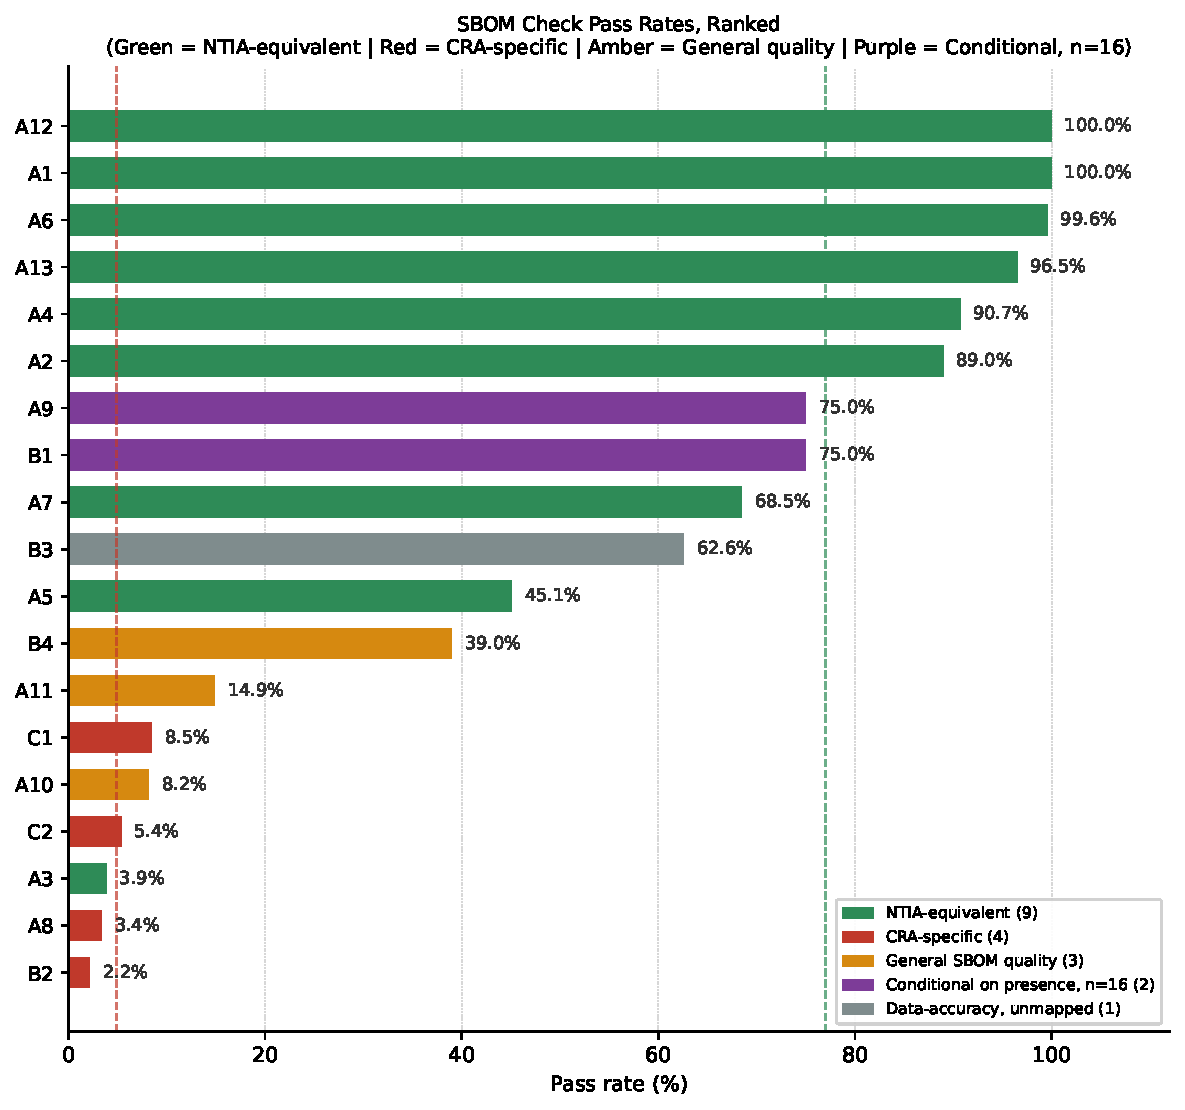
\includegraphics[width=0.85\textwidth]{figure1_check_pass_rates.pdf}
\caption{SBOM check pass rates, ranked from lowest to highest. Colours indicate requirements group: green = NTIA-equivalent; red = CRA-specific; amber = general SBOM-quality; purple = conditional on presence ($n=16$); grey = unmapped data-accuracy check (B3). Dashed lines mark the NTIA-equivalent (77.0\%) and CRA-specific (4.9\%) group averages. A12's 100\% pass rate is a corpus-construction artifact (\cref{sec:a12-caveat}) and is excluded from substantive interpretation.}
\label{fig:checkrates}
\end{figure}

Two patterns are immediately visible. First, the NTIA-equivalent checks cluster heavily toward the high end of the chart: six of the nine score above 68\%, including four above 89\%. Second, the four CRA-specific checks cluster tightly and uniformly at the low end of the ranking, with no exceptions: A8 (3.4\%), B2 (2.2\%), C1 (8.5\%), and C2 (5.4\%) span only a 6.3-percentage-point range, all comfortably below every NTIA-equivalent check except one. This tightness is itself notable: unlike the general-quality group, where B4's 39.0\% pass rate stands well above A10 and A11, the CRA-specific group shows no high-scoring outlier, suggesting the gap reflects a broad, consistent shortfall across all four genuinely CRA-grounded requirements rather than being driven by any single weak check.

The one notable exception within the NTIA-equivalent group is A3 (Supplier/originator identification), which scores 3.9\% -- the worst-performing NTIA-equivalent check by a wide margin, and within the same range as the CRA-specific group despite mapping exactly to NTIA's ``Supplier Name'' field. We discuss this finding, consistent with prior tool-accuracy literature \cite{muneza2025,halbritter2024}, in \cref{sec:a3-discussion}.

\subsection{The Vulnerability-Disclosure Gap: A8 Decomposition}
\label{sec:a8-decomp}

A8 (known vulnerabilities declared) shows an overall pass rate of 3.4\% (171 of 5,000 files). However, this figure combines two qualitatively different signals. Decomposing the 171 passing files:

\begin{itemize}
\item 16 files (0.32\% of the corpus) contain a non-empty, structured CycloneDX \texttt{vulnerabilities[]} array -- per-component, machine-readable vulnerability entries of the kind CRA Annex I's vulnerability-handling provisions would require in practice.
\item 155 files (3.10\% of the corpus) pass only via an SPDX \texttt{externalRefs} entry with \texttt{referenceCategory: SECURITY} -- typically a generic link to an advisory or security page, without structured per-vulnerability content.
\end{itemize}

In other words, 91\% of the SBOMs that nominally ``pass'' the vulnerability-declaration check do so via a generic link rather than actionable vulnerability data. The substantive, CRA-relevant figure is not 3.4\% but 0.32\% -- fewer than 1 in 300 SBOMs in our corpus. As discussed in \cref{sec:taxonomy}, A8 is the most directly CRA-grounded of our four CRA-specific checks; its near-total reliance on generic links rather than structured data is therefore the most regulatorily consequential single finding in this study.

\subsection{Conditional Finding: Quality Given Presence (A9, B1)}
\label{sec:conditional}

A9 (recognisable vulnerability-identifier format) and B1 (CVE identifiers validate against OSV.dev) are evaluated only on the 16 SBOMs identified above that contain structured \texttt{vulnerabilities[]} data. Among these 16 files:

\begin{itemize}
\item \textbf{A9:} 75.0\% use a recognisable identifier format (95\% CI: 50.5--89.8\%; $n=16$).
\item \textbf{B1:} 75.0\% have identifiers that successfully validate against the OSV.dev vulnerability database (95\% CI: 50.5--89.8\%; $n=16$).
\end{itemize}

We emphasise that both estimates carry substantial uncertainty given the small sample, with confidence intervals spanning roughly 40 percentage points; we report them as a preliminary, descriptive signal rather than a precise quality measure. With that caveat, the available evidence does not suggest that vulnerability data, when present, is markedly unreliable -- both point estimates fall well above chance and toward the upper half of their respective confidence intervals. The more statistically robust finding is one of presence: 99.68\% of SBOMs in our corpus contain no structured vulnerability data at all ($n=4{,}984$ of 5,000, a proportion estimated with high precision). We therefore characterise the vulnerability-disclosure gap as predominantly a problem of absence, with quality-given-presence remaining an open question warranting a larger sample in future work.

\subsection{Sensitivity Analysis: Tool Concentration}
\label{sec:sensitivity}

Eight tools account for roughly 93\% of the corpus, with cdxgen alone contributing 1,348 files (27.0\%) -- though, as discussed in \cref{sec:sampling}, the true cdxgen share is likely higher due to the ``Node.js module'' attribution artifact, making this and the following sensitivity figures conservative with respect to cdxgen's actual influence. To assess whether the headline gap is an artifact of tool concentration, we extend our sensitivity analysis beyond a single-tool exclusion to four progressively stricter scenarios: excluding cdxgen alone; excluding cdxgen and ``Node.js module'' together (the two largest labelled categories, addressing the possibility that their shared mislabelling masks a single dominant generator's influence); excluding the three largest tool categories cumulatively; and restricting the corpus to only those tools each contributing under 5\% of files individually -- an extreme test isolating the long tail of 46+ minor tools.

\begin{table}[t]
\centering
\caption{Sensitivity of the headline NTIA-equivalent/CRA-specific compliance gap to four tool-exclusion scenarios (Excl.\ = excluding; see \cref{sec:sensitivity} for scenario definitions).}
\label{tab:sensitivity}
\begin{tabular}{lrrrr}
\toprule
Corpus & $N$ & NTIA avg.\ & CRA avg.\ & Gap \\
\midrule
Full corpus & 5,000 & 77.0\% & 4.9\% & 72.2pp \\
Excl.\ cdxgen & 3,652 & 76.0\% & 6.3\% & 69.7pp \\
Excl.\ cdxgen + ``Node.js module'' & 2,735 & 76.4\% & 8.1\% & 68.3pp \\
Excl.\ top 3 tools\textsuperscript{a} & 2,112 & 74.3\% & 8.8\% & 65.6pp \\
Tools with $<$5\% individual share only & 819 & 77.5\% & 5.4\% & 72.1pp \\
\bottomrule
\end{tabular}
\\[2pt]
\raggedright\footnotesize\textsuperscript{a}cdxgen, ``Node.js module'', cyclonedx-php-composer.
\end{table}

The gap narrows somewhat as the most concentrated tool categories are removed (72.2pp $\rightarrow$ 65.6pp under the strictest three-tool exclusion) but remains substantial in every scenario, never falling below 65.6 percentage points. Most notably, when the corpus is restricted to only the long tail of tools each contributing under 5\% of files -- a scenario with no shared dependence on any dominant generator's defaults -- the gap returns to 72.1pp, essentially matching the full-corpus figure. This pattern is consistent with the headline result reflecting broad ecosystem-wide behaviour rather than the configuration choices of any single tool or small set of tools.

\subsection{Tool- and Format-Level Breakdown}
\label{sec:tool-format}

Pass rates vary substantially by tool across both the CRA-specific and general-quality groups. \Cref{tab:tool-breakdown} shows results for the five most common tools on a selection of checks, combining CRA-specific checks (A3, A8, B2, C1, C2) with the general-quality and data-accuracy checks (A11, B4, B3) for comparison.

\begin{table}[t]
\centering
\caption{Pass rates (\%) for the five most common tools in the corpus, across CRA-specific checks (A3, A8, B2, C1, C2) and general-quality/accuracy checks (A11, B4, B3) for comparison.}
\label{tab:tool-breakdown}
\begin{tabular}{lrrrrrrrr}
\toprule
Tool ($n$ files) & A3 & A8 & A11 & B2 & B4 & C1 & C2 & B3 \\
\midrule
cdxgen (1,348) & 1.6 & 0.1 & 4.1 & 2.1 & 8.6 & 0.1 & 1.9 & 65.7 \\
Node.js module (917)\textsuperscript{a} & 3.4 & 0.0 & 5.9 & 1.8 & 57.2 & 0.0 & 2.1 & 88.4 \\
cyclonedx-php-composer (623) & 0.0 & 0.0 & 85.4 & 1.4 & 30.0 & 0.0 & 20.9 & 1.8 \\
cyclonedx-gomod (502) & 0.0 & 0.0 & 0.0 & 1.6 & 17.3 & 0.0 & 0.0 & 97.6 \\
syft (445) & 15.1 & 34.8 & 0.9 & 0.4 & 76.3 & 83.8 & 0.0 & 15.7 \\
\bottomrule
\end{tabular}
\\[2pt]
\raggedright\footnotesize\textsuperscript{a}See \cref{sec:sampling,sec:threats} -- this label reflects a tool-attribution artifact; true generators are predominantly cdxgen ($\approx$68\%) and cyclonedx-php-composer ($\approx$20\%) of re-examined files.
\end{table}

syft is a clear outlier, scoring far above every other tool on A8 (34.8\%), B4 (76.3\%), and especially C1 (83.8\%) -- reflecting its typical use case of scanning container images and filesystems. As discussed in \cref{sec:related}, Yu et al.\ \cite{yu2024} find that major SBOM generators, including syft and trivy, produce inconsistent and incomplete output relative to one another even on identical inputs; we read syft's outlier status here as plausibly reflecting both its distinct use case (container/filesystem scanning, which naturally surfaces deployment-context and vulnerability signals that library-level generators do not) and, potentially, generator-level inconsistency of the kind Yu et al.\ document. Our corpus does not allow us to separate these two explanations, since we observe each SBOM only as generated, without a ground-truth comparison across generators for the same underlying software.

cyclonedx-php-composer stands out on A11 (licence per component, 85.4\%) -- now classified as a general-quality rather than CRA-specific check (\cref{sec:taxonomy}) -- reflecting PHP's Composer ecosystem convention of declaring per-package licence metadata.

Format-level comparison (\Cref{tab:format-breakdown}) shows SPDX-JSON substantially outperforming both CycloneDX variants on several checks despite representing only 5.5\% of the corpus.

\begin{table}[t]
\centering
\caption{Pass rates (\%) by SBOM format, for a representative subset of checks. A9 and B1 are evaluated only for CycloneDX-JSON files, consistent with their dependence on the CycloneDX \texttt{vulnerabilities[]} field.}
\label{tab:format-breakdown}
\begin{tabular}{lrrr}
\toprule
Check & CycloneDX-JSON (88.2\%) & CycloneDX-XML (6.3\%)\textsuperscript{a} & SPDX-JSON (5.5\%) \\
\midrule
A3 (supplier) & 2.6\% & 0.0\% & 26.7\% \\
A5 (dependencies) & 45.1\% & 0.0\% & 97.8\% \\
A7 (timestamp) & 69.4\% & 31.2\% & 97.1\% \\
A8 (vulnerabilities) & 0.4\% & 0.0\% & 56.8\% \\
A13 (format version) & 99.4\% & 52.9\% & 100.0\% \\
B4 & 36.8\% & 0.0\% & 65.4\% \\
C1 (deployment env.) & 6.9\% & 3.5\% & 39.6\% \\
A9 / B1 ($n=16$) & 75.0\% / 75.0\% & --- & --- \\
\bottomrule
\end{tabular}
\\[2pt]
\raggedright\footnotesize\textsuperscript{a}Subject to the component-count bypass and missing tool attribution described in \cref{sec:threats}.
\end{table}

\subsection{Tool Capability: Structured Vulnerability Data in the ``Other'' Tools}
\label{sec:existence-proof}

The 16 SBOMs containing structured \texttt{vulnerabilities[]} data are concentrated outside the top-8 tools, originating predominantly from trivy (a mainstream container/filesystem vulnerability scanner) and hoppr, with smaller contributions from grype, OSS Review Toolkit, and Debricked.

This finding demonstrates that mainstream, freely-available tooling capable of producing CRA-relevant structured vulnerability output exists, and is therefore more consistent with an adoption and configuration gap than a fundamental capability gap: most generators in our corpus do not appear to invoke or enable this functionality by default, even though tools that do so are readily available. We interpret this finding with caution, however, in light of Churakova et al.\ \cite{churakova2025}, who find that VEX-generation tools -- including trivy itself -- exhibit low cross-tool consistency (maximum pairwise Jaccard similarity of 69.4\% across the seven tools they evaluate, driven primarily by differing underlying vulnerability-database coverage). A tool's demonstrated capability to produce structured output, as we observe here, does not by itself establish that such output would be complete or consistent if adopted more broadly; the VEX/vulnerability-tooling ecosystem's broader immaturity, as documented by Churakova et al., suggests that closing this gap may require not only broader adoption of capable tools but also continued maturation of the underlying tools themselves.

\subsection{Summary of Key Findings}

\begin{enumerate}
\item SBOMs pass NTIA-equivalent checks at 77.0\% but the four genuinely CRA-specific checks at only 4.9\% -- a 72.2 percentage-point gap, statistically significant (Wilcoxon $p<0.001$).
\item This gap remains substantial (65.6--72.2pp) across a full range of tool-exclusion sensitivity scenarios, including when the corpus is restricted to tools individually contributing under 5\% of files.
\item The CRA vulnerability-disclosure gap is driven by near-total absence of structured data (0.32\%); the quality of that small fraction of data, while not obviously poor, is estimated imprecisely (95\% CI 50.5--89.8\%, $n=16$) and should be treated as preliminary.
\item A3 (supplier identification), an exact NTIA requirement, scores 3.9\% -- within the same range as the CRA-specific group, and consistent with prior tool-accuracy findings \cite{muneza2025,halbritter2024}.
\item Three general SBOM-quality checks (component integrity hashing, licence presence, licence validity), while not CRA-specific, show intermediate compliance (mean 20.7\%) -- better than the CRA-specific group but still well below NTIA-equivalent levels.
\item Mainstream tools (trivy, syft) demonstrate that CRA-relevant signals are achievable with existing, freely-available tooling, though documented inconsistency across VEX-generation tools \cite{churakova2025} tempers how far this finding can be generalised.
\end{enumerate}

\section{Discussion and Remediation Guidance}
\label{sec:discussion}

\subsection{Presence, Not Quality, Is the Primary Barrier}

The clearest implication of \cref{sec:results} is that the gap between current SBOM practice and CRA Annex I's vulnerability-disclosure requirements is, at minimum, predominantly a presence problem rather than a quality problem. The robust finding here is one of absence: 99.68\% of SBOMs in our corpus never reach the point of containing any structured vulnerability data to evaluate. Among the small fraction (0.32\%, $n=16$) that do, the available evidence does not suggest the data is markedly unreliable, though as discussed in \cref{sec:conditional}, this sub-finding rests on a sample too small to support a confident quality assessment in either direction.

A quality problem would call for better validation, linting, or correction of existing vulnerability metadata. A presence problem calls for something different: ensuring that SBOM-generation pipelines invoke vulnerability-scanning functionality and populate the relevant fields in the first place. \Cref{sec:existence-proof}'s tool-capability finding is consistent with this being substantially a configuration and pipeline-integration problem, since mainstream, freely-available tools capable of producing this data exist. This interpretation warrants some caution, however: Churakova et al.\ \cite{churakova2025} document that VEX-generation tools -- including trivy, one of the tools we identify as capable (\cref{sec:existence-proof}) -- are themselves inconsistent with one another, suggesting that even organisations that successfully enable vulnerability-scanning functionality may not obtain complete or mutually consistent results depending on tool choice. Separately, per the discussion in \cref{sec:cra-background}, some readings of CRA's vulnerability-coordination obligations -- including BSI TR-03183-2's guidance \cite{bsi2025} -- locate this information in separate VEX/CSAF documentation rather than within the SBOM itself; under that reading, the near-total absence of SBOM-embedded vulnerability data we observe would not by itself indicate non-compliance, provided equivalent VEX/CSAF documentation exists elsewhere. Our corpus, drawn from SBOM files alone, cannot determine whether such separate documentation exists for the manufacturers represented in our sample.

With these caveats, we suggest -- rather than conclude -- that organisations preparing for CRA Article 13 enforcement would benefit from auditing which stage of their SBOM and broader vulnerability-disclosure pipeline is expected to populate this information, whether within the SBOM or via accompanying VEX/CSAF documentation, and confirming that stage is actually in place.

\subsection{The A3 (Supplier) Finding: An Old Gap, Not Just a New One}
\label{sec:a3-discussion}

A3's 3.9\% pass rate complicates the paper's central framing, though it is not, on reflection, an anomaly so much as a confirmation of a known issue. A3 -- supplier or originator identification -- is one of NTIA's original seven Minimum Elements from 2021, with no novel CRA-specific content, yet it is the worst-performing check in the entire NTIA-equivalent group, falling within the same range as our CRA-specific checks. This is consistent with prior work: Muneza et al.\ \cite{muneza2025} report substantial tool-to-tool variation in NTIA field compliance, and Halbritter and Merli \cite{halbritter2024} find that no SBOM tool fully satisfies NTIA requirements across the languages they evaluate. Our finding adds corpus-scale confirmation, at a single-field level, that supplier identification specifically -- as distinct from NTIA compliance in aggregate -- remains a persistent, longstanding gap rather than a newly discovered one.

Tool maintainers and SBOM consumers should not treat a high aggregate NTIA score as evidence that all seven original fields are well-populated; A3 in particular warrants individual attention regardless of CRA's additional requirements.

\subsection{Format Choice Has First-Order Effects on CRA-Readiness}

SPDX-JSON SBOMs substantially outperform CycloneDX-JSON on several CRA-relevant checks. Most strikingly, A8 reaches 56.8\% for SPDX-JSON versus 0.4\% for CycloneDX-JSON. However, as discussed in \cref{sec:a8-decomp}, the great majority of SPDX's A8 advantage reflects generic \texttt{externalRefs}/SECURITY links rather than structured vulnerability content, while the structured-data path (A9/B1) is exclusively a CycloneDX phenomenon in our corpus. This points to a genuine trade-off rather than a straightforward format ranking: CycloneDX has the better-suited field for CRA's vulnerability-handling provisions (its \texttt{vulnerabilities[]} array), yet that field sits empty in 99.64\% of CycloneDX-JSON files in our corpus; SPDX's generic security references are populated more often but, as currently used, carry comparatively less actionable content. Bangash et al.'s \cite{bangash2026} ecosystem-level comparison -- finding CycloneDX tooling shows higher developer engagement while SPDX benefits from broader tool availability -- offers a plausible structural explanation for this divergence: a more actively developed CycloneDX tooling ecosystem may simply not yet have converged on populating its security-specific fields by default, despite the format affording the capability.

\subsection{Tool-Specific Observations}

syft's outlier status on C1 (83.8\% vs.\ near-0\% for all other tools) reflects its typical use case of scanning container images and filesystems, naturally yielding OS-package entries and container-level metadata; as noted in \cref{sec:tool-format}, we cannot fully separate this use-case explanation from the possibility of broader generator-level inconsistency documented by Yu et al.\ \cite{yu2024}. With that caveat, this finding points to an important nuance: C1's low overall score partly reflects that the majority of the corpus consists of library-level SBOMs for which ``deployment environment'' may not be a meaningful per-SBOM attribute in the first place, rather than a uniform failure of tooling to disclose this information when it is relevant. For organisations assembling final, deployable products, the more relevant comparison point may be syft's 83.8\%, suggesting this information can be readily available when the SBOM is generated at the image/deployment level -- though we would caution against treating this as a general claim about tool capability given only one tool in our corpus shows this pattern strongly.

cyclonedx-php-composer's strong performance on A11 (licence presence, 85.4\% -- now classified as a general-quality rather than CRA-specific check; \cref{sec:taxonomy}) shows that licence-per-component metadata is achievable at near-universal rates within at least one ecosystem's tooling conventions, suggesting that ecosystem-level norms can substantially shape SBOM completeness independent of the generator tool's own design.

\subsection{Practical Remediation Priorities}

The following priorities follow from our findings but should be read as plausible, evidence-informed suggestions rather than conclusions our data can fully establish; we order them by how directly our findings support each one.

\begin{enumerate}
\item \textbf{Consider enabling vulnerability scanning in the SBOM pipeline, or ensuring equivalent VEX/CSAF documentation exists.} Structured vulnerability data is largely absent (0.32\%) in our corpus. Given that mainstream tools capable of populating it exist (\cref{sec:existence-proof}), integrating such a step is a plausible high-impact intervention -- though, as discussed in \cref{sec:discussion}, this presumes vulnerability information is intended to live within the SBOM rather than (or in addition to) separate VEX/CSAF documentation, and organisations should confirm which interpretation applies to their compliance strategy.
\item \textbf{Audit supplier/originator metadata (A3).} As an exact NTIA field with near-total absence (3.9\%) in our corpus, and consistent with prior tool-accuracy findings \cite{muneza2025,halbritter2024}, this appears to be both a tractable improvement and foundational to supply-chain accountability independent of CRA-specific obligations.
\item \textbf{Consider matching SBOM generation level to the requirement.} For deployment-environment and support-period information (C1, C2), our data suggests -- via syft's outlier performance on C1 -- that generating SBOMs at the image/deployment level for final products may surface this context more readily than library-level generation, though we note this observation rests on a single tool's behaviour in our corpus.
\item \textbf{Address end-of-life and support-period disclosure (B2, C2).} These score lowest among our CRA-specific checks (2.2\% and 5.4\%); organisations may wish to supplement automated SBOM-embedded checks with internally-maintained component lifecycle records, particularly given that CRA's underlying obligation does not clearly require this information to be SBOM-embedded in the first place (\cref{sec:taxonomy}).
\item \textbf{Consider format choice deliberately, with awareness of ecosystem-level trade-offs.} CycloneDX's native vulnerability-array support represents under-exploited capability in our corpus; SPDX's \texttt{externalRefs} conventions see broader, if shallower, adoption. Bangash et al.'s \cite{bangash2026} finding that the two formats' tooling ecosystems differ in engagement and maturity (\cref{sec:discussion}) suggests this trade-off may shift as both ecosystems develop.
\end{enumerate}

\section{Threats to Validity}
\label{sec:threats}

We group the following threats into three categories to aid navigation: corpus representativeness (Threats 1, 3, 5, 7), tool attribution and taxonomy grounding (Threats 2, 4, 9), and measurement and implementation detail (Threats 6, 8, 10--13). Numbering follows the order in which threats are introduced below, and is preserved across categories so that cross-references elsewhere in the paper (e.g., ``Threat 4'') remain unambiguous.

\begin{enumerate}[label=\arabic*.,leftmargin=*]
\item \textbf{[Representativeness] Corpus represents open-source tooling output, not the CRA-regulated population directly.} As discussed in \cref{sec:introduction,sec:sampling}, our corpus is drawn from public code-hosting platforms via the Software Heritage Archive, and predominantly captures open-source, developer-facing SBOMs. CRA Article 13 governs manufacturers placing commercial products with digital elements on the EU market. Such manufacturers' internal SBOMs are typically confidential technical documentation, not artefacts committed to public repositories, and are therefore unlikely to be represented in our corpus. We treat our findings as a measurement of what current, widely-used open-source SBOM tooling produces by default -- directly informative for any manufacturer relying on this tooling, which we expect to be common, but not a direct sample of CRA-regulated manufacturer practice. We are not aware of a publicly available dataset of manufacturer-internal SBOMs that would permit a direct sample of the regulated population. Assembling such a dataset is an important direction for future work.

\item \textbf{[Taxonomy grounding] CRA-specific check grounding varies in strength.} As detailed in \cref{sec:taxonomy}, our four CRA-specific checks are not equally well-grounded in CRA Annex I text. A8 and B2 correspond to identifiable CRA provisions and are supported by independent regulatory analysis \cite{ruohonen2025timmers,ruohonen2025gdpr}; C1 and C2 reflect a more speculative operationalisation of CRA's broader transparency intent, and we are not aware of a specific Annex I clause or published analysis mapping them directly to SBOM content. Readers should weight findings involving C1 and C2 accordingly. Separately, whether vulnerability information (A8) and lifecycle status (B2) must be embedded within the SBOM itself, as our checks assume, or may instead be satisfied through separate VEX/CSAF documentation, is an open architectural question on which authoritative guidance is not unanimous (\cref{sec:cra-background}); BSI TR-03183-2 \cite{bsi2025} favours the latter reading.

\item \textbf{[Representativeness] Corpus sampling is not exactly reproducible.} As described in \cref{sec:sampling}, our 5,000-file sample was drawn via Python's \texttt{random.shuffle()} applied to the qualifying-file list without a fixed random seed. While the resulting sample is a valid random subset of the 15,000 qualifying files identified, and we have no specific reason to expect it is unrepresentative, an independent re-run of our sampling procedure would select a different 5,000-file sample. We did not assess whether results are stable across alternative random samples; doing so is a natural extension for future work.

\item \textbf{[Tool attribution] Tool attribution artifact affecting approximately 18\% of the corpus.} As detailed in \cref{sec:sampling}, files labelled ``Node.js module'' ($n=917$, 18.3\% of corpus) reflect a tool-extraction artifact rather than a genuine generator category; a post-hoc audit found the true generators to be predominantly cdxgen and cyclonedx-php-composer. This means the true corpus share of these two tools is materially higher than reported throughout this paper, and our tool-concentration sensitivity analysis (\cref{sec:sensitivity}) should be read as conservative with respect to cdxgen's actual influence. We retain the original attribution throughout for consistency and do not recompute tool-level findings in this version of the paper; the headline NTIA-equivalent/CRA-specific gap (\cref{sec:headline}) is unaffected, since it is computed per-check across the full corpus independent of tool label.

\item \textbf{[Representativeness] Tool concentration.} Eight tools account for approximately 93\% of the corpus (a figure itself affected by Threat 4 above). \Cref{sec:sensitivity} reports an extended sensitivity analysis across four exclusion scenarios, including cumulative exclusion of the three largest tool categories and restriction to tools with under 5\% individual corpus share; the headline gap remains within 65.6--72.2 percentage points across all scenarios, providing stronger robustness evidence than a single-tool exclusion would offer.

\item \textbf{[Measurement detail] Implementation sampling caps within Tier B checks.} As noted in \cref{sec:implementation}, all four Tier B checks apply per-SBOM sampling caps when querying external APIs (20 vulnerability entries for B1; 30 components for B2 and B4; 15 PURLs for B3) to bound runtime. For SBOMs with component or vulnerability counts exceeding these caps, the reported result reflects a sample rather than the complete set of declared data. Given that our corpus's typical declared-dependency counts (\cref{sec:results}, A5 statistics) are generally well below these thresholds, we expect this to affect a minority of files, concentrated among those with unusually large component lists; we did not separately quantify the magnitude of this effect.

\item \textbf{[Representativeness] Sampling methodology.} The 5,000-file corpus is drawn from the first 5,000 files, in shuffle order, among 15,000 files meeting structural-validity criteria, identified via a scan of the 78,612-file archive that stopped once those 15,000 qualifying files were found (approximately 22,800 files examined in total; approximately 55,800 never examined). Because the full file list was shuffled prior to traversal, both the examined and retained subsets are random with respect to the original archive ordering, subject to Threat 3 above regarding exact reproducibility.

\item \textbf{[Measurement detail] CycloneDX-XML component-count bypass and tool-attribution gap.} The $\geq$5-component threshold was not applied to CycloneDX-XML files (6.3\% of the corpus, $n=315$) due to parser limitations at filtering time; such files were assigned a placeholder component count of 99 and were not subject to tool-name extraction (all CycloneDX-XML files are therefore attributed to ``unknown'' or omitted from tool-level analysis). This may partly explain CycloneDX-XML's generally low scores across multiple checks in \cref{tab:format-breakdown}, and means CycloneDX-XML files contribute no information to the per-tool breakdown in \cref{tab:tool-breakdown}.

\item \textbf{[Tool attribution] The ``unknown'' tool category ($n=346$, 6.9\%) was not independently audited.} Unlike the ``Node.js module'' category (Threat 4), we did not perform a post-hoc audit of files attributed to ``unknown'' to determine whether this label similarly conflates multiple distinct generators or genuinely reflects unparseable tool metadata. Given the parsing issue identified for ``Node.js module'', we cannot rule out that some fraction of the ``unknown'' category reflects a similar attribution artifact rather than genuinely absent tool metadata.

\item \textbf{[Measurement detail] A8 vulnerability-declaration semantics -- composite measure.} A8's 3.4\% pass rate combines two qualitatively different signals: SBOMs with structured, machine-readable vulnerability data (0.32\%, $n=16$) and SBOMs with only a generic security-reference link (3.10\%, $n=155$). A8 should be interpreted alongside the decomposition in \cref{sec:a8-decomp}.

\item \textbf{[Measurement detail] A9/B1 conditional measurement and small-sample uncertainty ($n=16$).} One additional file had blank A8/A9/B1 values due to a parsing artifact and was excluded from the $n=16$ group; including it would not change the reported point estimates. More substantively, as discussed in \cref{sec:conditional}, both A9 and B1 carry wide 95\% confidence intervals (50.5--89.8\%) given this small sample; we treat the corresponding quality-given-presence finding as preliminary.

\item \textbf{[Measurement detail] C1/C2 heuristic precision and binary scoring.} Tier C checks rely on multi-signal structural inference rather than ground-truth validation, and -- unlike Tier A/B checks -- return binary PASS/FAIL rather than a graded PARTIAL/SKIP outcome (\cref{sec:taxonomy-tiers}). C1's low overall score (8.5\%) partly reflects that ``deployment environment'' may not be a well-defined attribute for library-level SBOMs, which dominate our corpus. C2's 5.4\% should be read as a conservative (upper-bound) estimate of declared support-period information.

\item \textbf{[Measurement detail] B2 external data-source coverage.} B2's 2.2\% pass rate partly reflects the coverage limitations of the endoflife.date API, which provides strongest coverage for major language runtimes and may under-evaluate less-common component types. Tier B checks were executed against external APIs across 13--14 June 2026 (\cref{sec:implementation}); results reflect the state of these continuously-updated data sources at that time and may differ under re-execution.
\end{enumerate}

\section{Conclusion}
\label{sec:conclusion}

We set out to answer an empirical question that, despite a growing body of SBOM-quality literature, had not yet been directly addressed: how ready is the output of current, widely-used open-source SBOM tooling for the additional security-disclosure requirements that CRA Annex I introduces beyond the NTIA Minimum Elements baseline? The answer, measured across 5,000 SBOMs drawn from 1,782 code-hosting forges, is that current tooling is poorly prepared: the four requirements most directly grounded in CRA Annex I text are met at rates not meaningfully different from a complete absence of compliance.

NTIA-equivalent checks pass at 77.0\% on average -- a reasonable baseline, though with notable individual gaps (A3, supplier identification, scores just 3.9\%, consistent with prior tool-accuracy literature \cite{muneza2025,halbritter2024}). The four checks most directly grounded in CRA Annex I -- vulnerability declaration, component end-of-life status, deployment-environment inferability, and security-support-period disclosure -- pass at just 4.9\% on average, a gap of 72.2 percentage points that a Wilcoxon signed-rank test confirms is statistically significant ($p<0.001$). This gap remains substantial (65.6--72.2 percentage points) across an extensive range of tool-exclusion sensitivity analyses, including when the corpus is restricted to tools each contributing under 5\% of files individually, indicating the result reflects broad ecosystem behaviour rather than the configuration choices of any one dominant generator. With CRA Article 13's SBOM obligations taking effect in September 2026 -- and full enforcement following in December 2027 -- this gap represents a concrete and immediate preparation challenge for organisations relying on current open-source tooling to produce or inform SBOMs for products placed on the EU market, while we note this corpus reflects open-source tooling output rather than a direct sample of CRA-regulated manufacturers' internal SBOM practice (\cref{sec:threats}).

The nature of the gap matters as much as its size. As shown in \cref{sec:a8-decomp,sec:conditional}, the vulnerability-disclosure gap is overwhelmingly one of absence (99.68\%) rather than fidelity: among the small fraction (0.32\%, $n=16$) of SBOMs that do carry structured data, the available evidence does not suggest it is markedly unreliable, though this sub-finding rests on a sample too small to support a confident conclusion either way. The absence, not the accuracy, of vulnerability data is therefore the binding constraint. This finding points toward pipeline-configuration strategies -- integrating tools such as trivy, which already produces CRA-relevant structured output -- as a plausible remediation direction, though documented inconsistency across vulnerability-scanning tools \cite{churakova2025} means broader adoption alone may not fully resolve the gap, and whether vulnerability data is required within the SBOM at all, as opposed to separate VEX/CSAF documentation, remains an open architectural question on which authoritative guidance is not unanimous (\cref{sec:cra-background}).

Beyond the headline gap, four further findings -- detailed in \cref{sec:results} and summarised in its closing list -- bear on remediation. The persistence of the A3 supplier-identification gap shows that a five-year-old NTIA requirement remains as poorly satisfied as our CRA-specific checks. A format-level trade-off separates CycloneDX, whose \texttt{vulnerabilities[]} array is the better-suited field for CRA's vulnerability-handling provisions yet sits empty in 99.64\% of CycloneDX-JSON files, from SPDX, whose more broadly (if shallowly) populated \texttt{externalRefs} conventions carry less structured content -- plausibly linked to differences in the two formats' tooling-ecosystem maturity. syft's 83.8\% pass rate on deployment-environment inferability, versus near-zero for all other tools, illustrates that CRA-relevant signals can be readily available when SBOMs are generated at the image/deployment level, though we draw this conclusion cautiously given it rests on a single tool's behaviour in our corpus. Finally, three general SBOM-quality checks not uniquely specific to CRA -- component integrity hashing, licence presence, and licence validity -- show intermediate compliance (mean 20.7\%), suggesting current tooling is somewhat more attentive to general supply-chain-integrity practice than to CRA-specific disclosure obligations specifically.

This study provides a dated, quantitative baseline -- 77.0\% / 4.9\% / 72.2pp -- drawn from SBOMs collected through approximately October 2024 and evaluated in June 2026, against which future work can measure whether the tooling ecosystem adapts ahead of and following CRA's September 2026 and December 2027 enforcement milestones. Measuring whether and how quickly the gap narrows, which tools and ecosystems lead or lag, whether the adoption-gap interpretation holds as more generators add vulnerability-scanning integration by default, and -- perhaps most importantly -- whether a corpus more directly representative of CRA-regulated commercial manufacturers shows a similar or different pattern, are natural and, we believe, valuable extensions of the empirical baseline this study establishes.

\bibliographystyle{plain}
\bibliography{references}

\end{document}
